\section{The Isomorphism Theorems.}
\label{section1}

\begin{theorem}[The First Isomorphism Theorem]\label{3.4.1}
    Let $G$ and  $H$ be groups and  $\phi:G \rightarrow H$ a homomorphism. Then
    $\ker{\phi} \unlhd G$ and $\faktor{G}{\ker{\phi}} \simeq \phi(G)$.
\end{theorem}
\begin{proof}
    Let $K=\ker{\phi}$ by lemma \ref{3.1.5}, we have $gK=Kg$, so  $K$ is normal
    in  $G$.

    Now consider $\psi:\faktor{G}{K} \rightarrow G$ by $gK \rightarrow g$. We
    have that $\psi$ is a homomorphism, moreover, it is $1-1$. Notice also that
    the $\phi:G \rightarrow \phi(G)$ is onto. Then form the map
    $\Phi:\faktor{G}{K} \rightarrow \phi(G)$ by taking $\Phi = \phi \circ \psi$.
    That is  $\Phi:gK \rightarrow \phi(g)$. Then, $\Phi$ is a $1-1$ homomorphism
    of  $\faktor{G}{K}$ onto $\phi(G)$; moreover it is well defined, for if
    $gK=g'K$, then  $g=g'k$, then  $\phi(g)=\phi(g')\phi(k)=\phi(g')$. This
    establishes the result.
\end{proof}
\begin{corollary}
    $[G : \ker{\psi}] = \ord{\phi(G)}$.
\end{corollary}
 \begin{figure}[h]
     \centering
     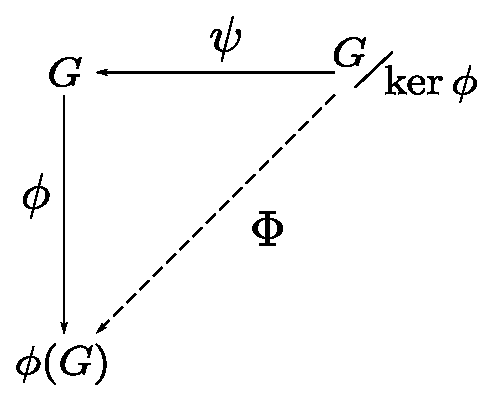
\includegraphics[scale = 0.5]{Figures/Chapter3/first_iso_thm.eps}
     \caption{The First Isomorphism Theorem}
     \label{fig_3.2}
 \end{figure}

\begin{theorem}[The Second Isomorphism Theorem]\label{3.4.4}
    Let $G$ be a group and  $A,B \leq G$ such that  $A \leq N(B)$. Then $AB \leq
    B$,  $B \unlhd AB$,  $A \cap B \unldh A$, and  $\faktor{AB}{B} \simeq
    \faktor{A}{A \cap B}$
\end{theorem}
\begin{proof}
    By the corollary to lemma \ref{3.3.7}, $A \leq N(B)$ implies that $AB \leq
    G$. Moreover, since  $B \lew N(B)$, $AB \leq N(B)$. Then
    $(ab)B\inv{(ab)}=abB\inv{b}\inv{a}=aB\inv{a}$, and since $A \leq N(B)$,
    $aB\inv{a} \subseteq B$, making $B \unlhd AB$.

    Now consider the map $\phi:A \rightarrow \faktor{AB}{B}$ by $\phi:a
    \rightarrow aB$. Since coset mutliplication is well defined, so is $\phi$,
    moreover, notice that  $\phi$ is a homomorphism, and is onto. Notice then
    that  $\ker{\phi}=\{a \in A : aB=B\}$, then $a \in B$, necessarily, so
    $\ker{\phi}=A \cap B$. Therefor, by the first isomorphism theorem, we get
    that $\faktor{AB}{B} \simeq \faktor{A}{A \cap B}$.
\end{proof}
\begin{remark}
    Notice that $\phi=\Phi|_{A}:AB \rightarrow \faktor{AB}{B}$.
\end{remark}
\begin{remark}
    The second isomorphism theorem states that if $A$ and $B$ are nontrivial
    subgroups of $G$  (i.e. $A,B \neq \vbrack{e}, G$), then the lattice of $G$
    contains the following sublattice described in figure \ref{fig_3.3}.
\end{remark}

\begin{figure}[h]
    \centering
    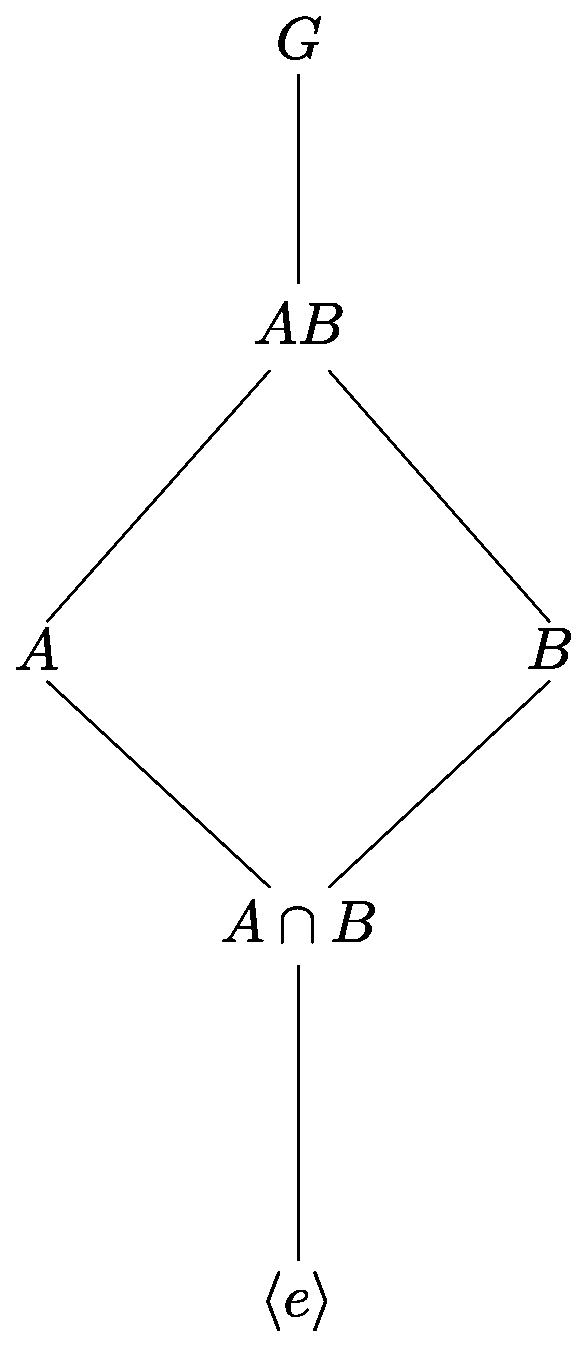
\includegraphics[scale = 0.3]{Figures/Chapter3/second_iso_thm.eps}
    \caption{The Second Isomorphism Theorem}
    \label{fig_3.3}
\end{figure}

\begin{theorem}[The Third Isomorphism Theorem]\label{3.4.3}
    Let $G$ be a group and let  $H \unlhd G$ and  $K \unlhd G$ such that  $H
    \leq K$. Then $\faktor{K}{H} \unlhd \faktor{G}{H}$, and
    $\faktor{G/H}{K/H} \simeq \faktor{G}{K}$.
\end{theorem}
\begin{proof}
    Notce that $kH=Hk$ for any $k \in K \leq G$. So that  $H$ is normal in  $K$.
    Now for all $gH \in \faktor{G}{H}$, we have $gHkH\inv{gH}=gk\inv{g}H=k'H$,
    since $K \unlhd G$. Now, we have that $gk\inv{g}=k'$, making $gk \in k'H$,
    and consequentially  $k \in k'H$, so that  $kH=k'H$. Thus we have
    $gk\inv{g}H \subseteq kH$, thus this makes $\faktor{K}{H} \unldh
    \faktor{G}{H}$.

    Now consider the map $\phi:\faktor{G}{H} \rightarrow \faktor{G}{K}$, by
    taking $gH \rightarrow gK$. We have that $\phi$ is a  $1-1$ homomorphism of
     $\faktor{G}{H}$ into $\faktor{G}{K}$. Moreover, it is well defined, since
     if $gH=g'H$, then $g=g'h$, and since $H \leq K$,  $g'h \in K$, so that
     $gK=g'K$.

     Notice then that  $\ker{\phi}=\{gH \in \faktor{G}{H} : gK=K\}=\{gH \in
         \faktor{G}{H} : g \in K\}=\faktor{K}{H}$. By the first isomorphism
         theorem, we have
         \begin{equation*}
             \faktor{G/H}{K/H} \simeq \faktor{G}{K}
         \end{equation*}
\end{proof}
\begin{remark}
    What this theorem says is that we obtain no new infromation upon taking
    quotients groups of quotient groups.
\end{remark}

\begin{theorem}[The Fourth Isomorphism Theorem]\label{3.4.2}
    let $G$ be a group and  $N \unlhd G$. Then there is a  $1-1$ mapping of the
    set of all subgroups  $A \leq G$ containing $N$ onto the set of subgroups
    $\faktor{A}{N}$ of $\faktor{G}{N}$. In particular, any subgroup of
    $\faktor{G}{N}$ is of the form $\faktor{A}{N}$, and the mapping has the
    following properties.
    \begin{enumerate}
        \item[(1)] $A \leq B$ if, and only if  $\faktor{A}{N} \leq \faktor{B}{N}$.

        \item[(2)] If $A \leq B$, then  $[B:A]=[\faktor{B}{N} : \faktor{A}{N}]$.

        \item[(3)] $\faktor{\vbrack{A,B}}{N}=\vbrack{\faktor{A}{N},
            \faktor{B}{N}}$.

        \item[(4)] $\faktor{A \cap B}{N}=\faktor{A}{N} \cap \faktor{B}{N}$.

        \item[(5)] $A \unlhd G$ if, and only if  $\faktor{A}{N} \unlhd
            \faktor{G}{N}$.
    \end{enumerate}
\end{theorem}
\begin{remark}
    What this theorem tells us is how to identify the lattice of subgroups of
    $\faktor{G}{N}$, which is embedded into the lattice of subgroups of $G$.
\end{remark}

\begin{example}\label{3.7}
    \begin{enumerate}
        \item[(1)] Let $N=\vbrack{-1} \unlhd \Hb$. Since
            $\faktor{\Hb}{\vbrack{-1}} \simeq V_4$, the lattice of
            $\faktor{\Hb}{\vbrack{-1}}$ is identical to that of $V_4$.

        \item[(2)] The lattice of $\faktor{D_8}{\vbrack{r^2}}$ is given by
            figure \ref{fig_3.4}. The lattice of the quotient group is
            represented by solid lines, while the rest of the lattice of $D_8$
            is represented by dotted lines.

            \begin{figure}[h]
                \centering
                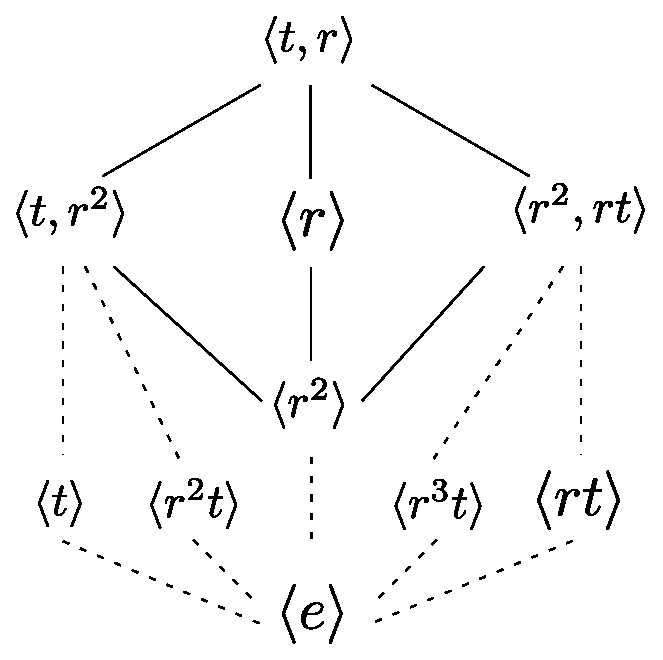
\includegraphics[scale = 0.5]{Figures/Chapter3/D_8_quotient_lattice.eps}
                \caption{The Lattice of subroups of $\faktor{D_8}{\vbrack{r^2}}$
                in the lattice of subgroup of $D_8$.}
                \label{fig_3.4}
            \end{figure}
            Notice also that $\faktor{D_8}{\vbrack{r^2}} \simeq V_4$.
    \end{enumerate}
\end{example}
